\section{System}\label{sec:System}
\todo[inline, color=red]{Vera}

\subsection{Lighting Model}\label{sec:lightingmodel}
\todo[inline, color=red]{Vera}

\subsection{Contours}\label{sec:contours}
\todo[inline, color=red]{Vera}
\subsubsection{Find Contours}\label{sec:findContours}
\todo[inline, color=red]{Vera}
\begin{figure}[H] 
	\center 
	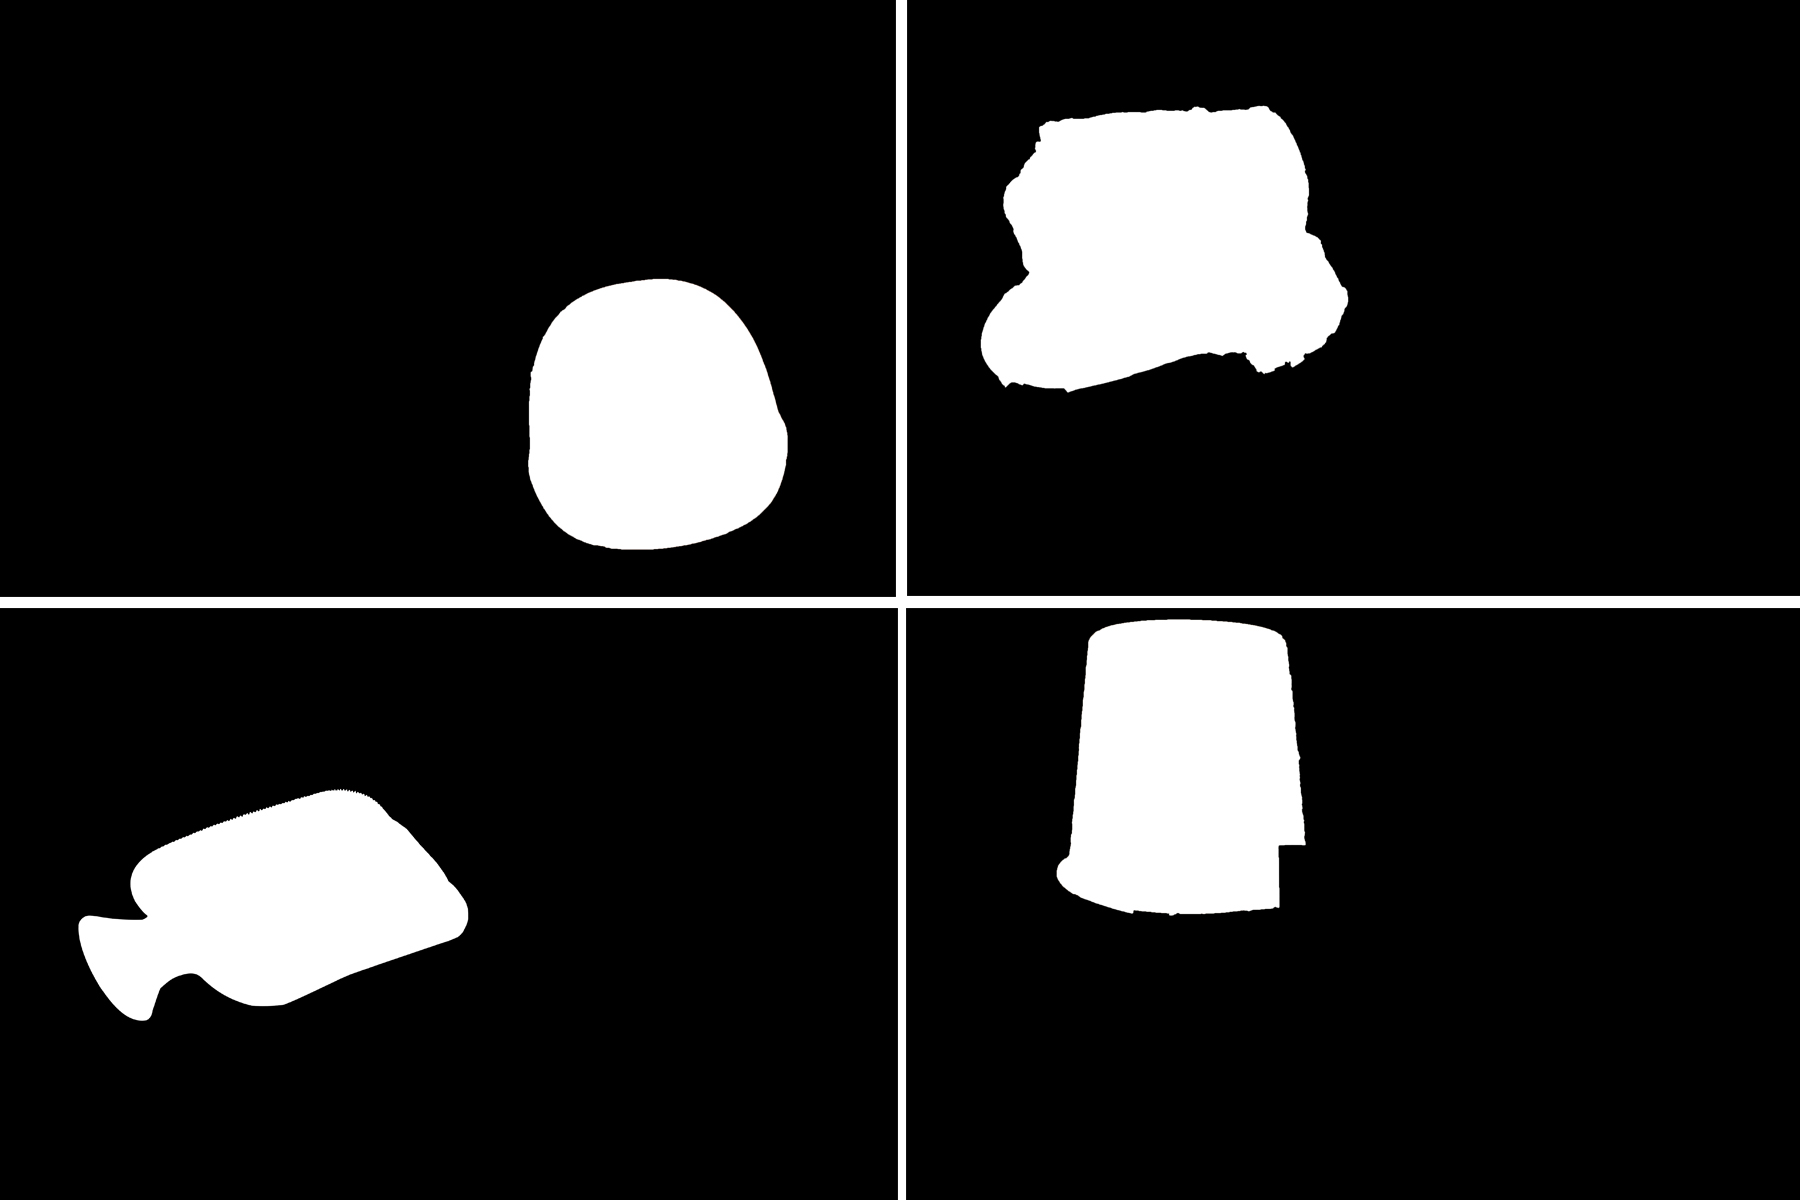
\includegraphics[width=12cm]{Images/batch1_mask.jpg}			
	\caption[Bildunterschrift]{Bildunterschrift.}
	\label{fig:batch1mask}
\end{figure}

\begin{figure}[H] 
	\center 
	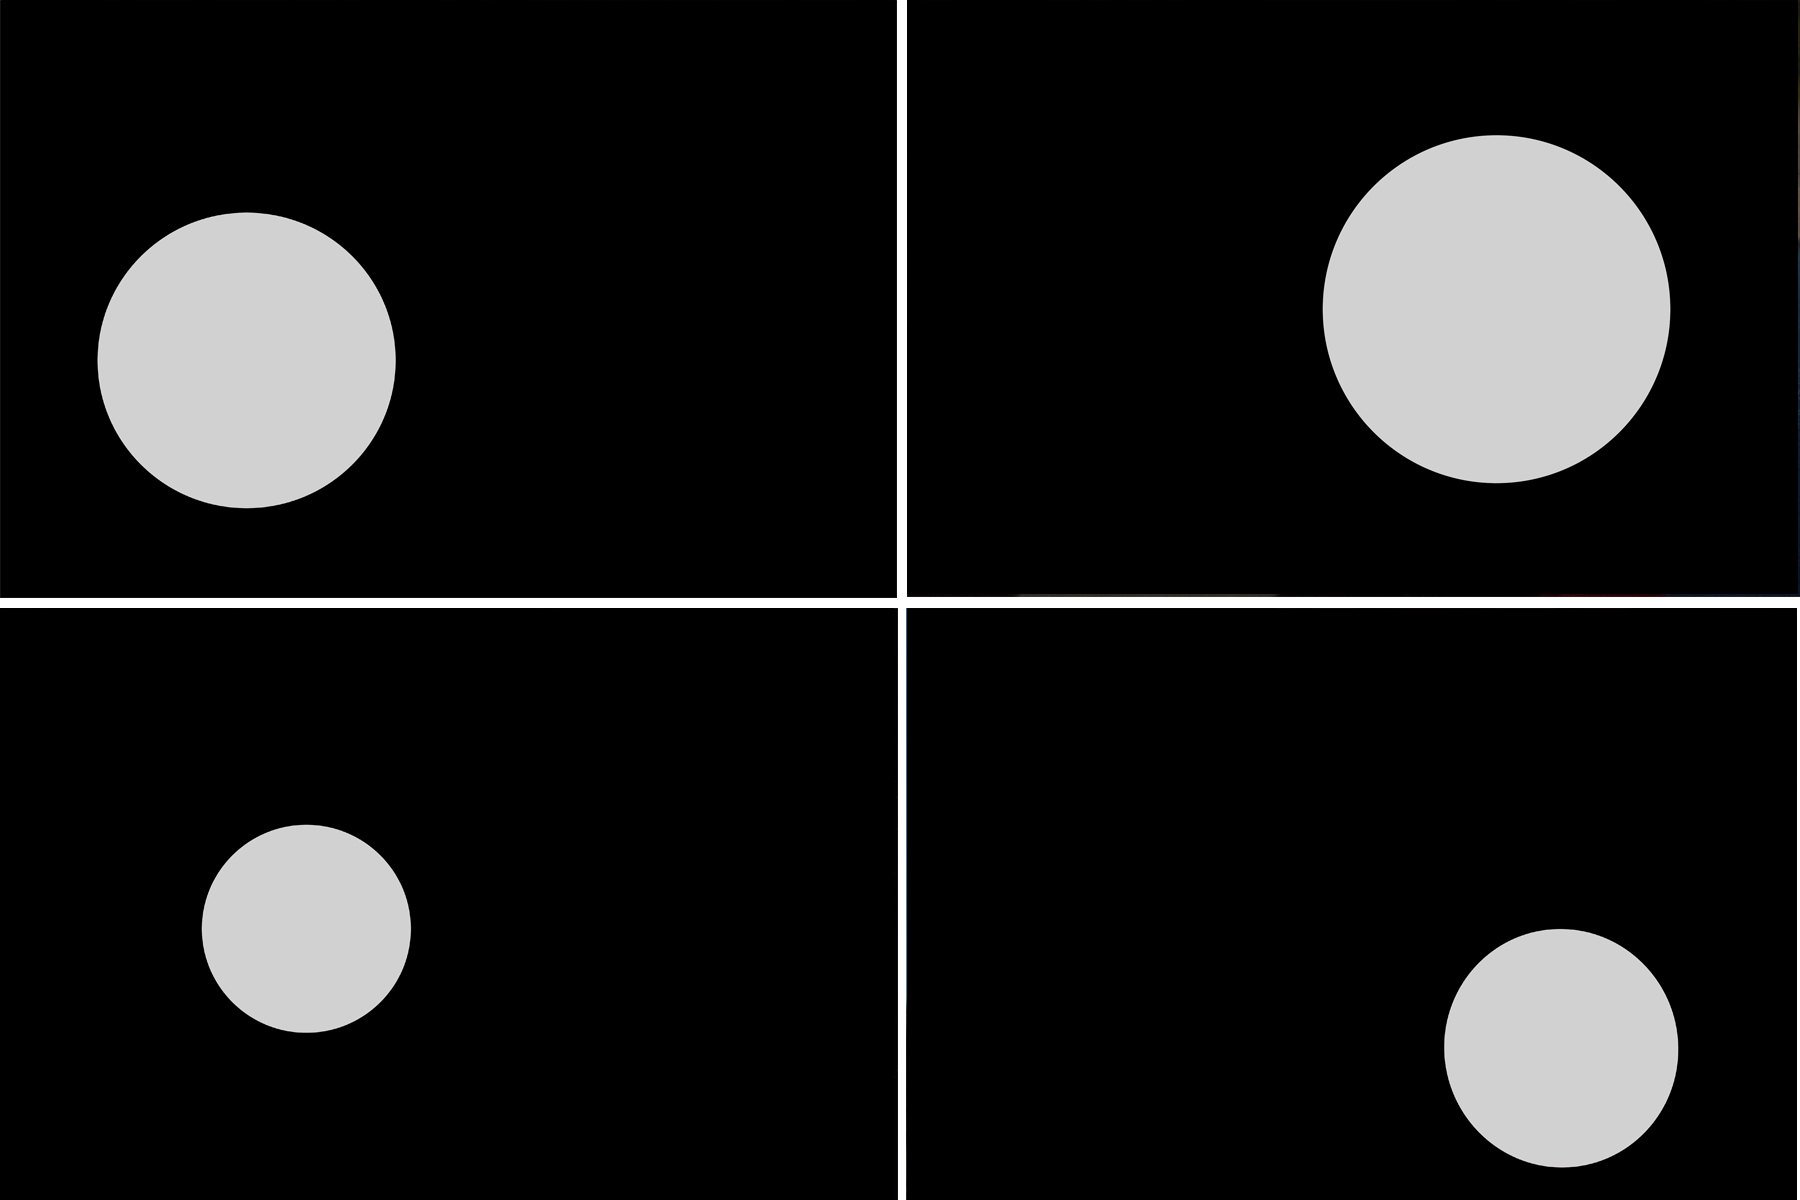
\includegraphics[width=12cm]{Images/batch2_mask.jpg}			
	\caption[Bildunterschrift]{Bildunterschrift.}
	\label{fig:batch2mask}
\end{figure}

\subsection{Subcontours}\label{sec:subcontours}
\todo[inline, color=red]{Vera}

\subsection{Different Approaches}\label{sec:approaches}
\todo[inline, color=red]{Laura}

\subsubsection{1. Approach: One Lightvector}\label{sec:appOne}
\todo[inline, color=red]{Laura}

\subsubsection{2. Approach: Averaging Lightvectors}\label{sec:appTwo}
\todo[inline, color=red]{Laura}

\subsubsection{3. Approach: Lightvector with highest Intensity}\label{sec:appThree}
\todo[inline, color=red]{Laura}


\newpage